\chapter{Minimalflächen\label{chapter:thema}}
\lhead{Minimalflächen}
\begin{refsection}
\chapterauthor{Nadja Rutz und Ambroise Suter}

\section{Einleitung}
%\rhead{Einleitung}

Flach aber trotzdem krumm!

Schon im Kindesalter lernen wir den Begriff der Krümmung kennen, doch gerade im mehrdimensionalen Raum gestaltet sich die Vorstellung und Berechnung von Krümmung als nicht ganz einfach. 

Die Menschheit brauchte mehrere Jahrtausende um herauszufinden, dass die Erde nicht flach sondern gekrümmt ist. 
Ähnliche Diskussionen kamen auch in der Kosmologie des Universums auf.
Viele Experimente zeigen, dass das Universum Flach ist. 
Je nach intrinsischer (innerer) und extrinsischer (äusser) Krümmung kann ein Raum aber auch flach sein wenn er extrinsisch gekrümmt ist.


\section{Problemstellung}
%\rhead{Problemstellung}

Minimalflächen haben eine mittlere Krümmung von Null. 

In diesem Kapitel werden zuerst verschiedene Krümmungsarten von Flächen vorgestellt, um anschliessend den Spezialfall der Minimalflächen genauer betrachten zu können. 
Zur Illustration werden einige Beispiele von Minimalflächen gerechnet. 
Als Vorstellungshilfe dienen oft nicht geschlossene Seifenfilme da diese von Natur aus  Minimalflächen erzeugen.


\subsection{Krümmung einer Fläche}
\index{Krümmung einer Fläche}

Intuitiv ist Krümmung einer Fläche für uns ein Mass der Abweichung eines Objekts im Bezug zu einer flachen Fläche. 

Die Krümmung einer Fläche im Punkt P kann in der Mathematik indirekt durch die Hauptkrümmungsradien $R1$ und $R2$ ausgedrückt werden. 
Die Hauptkrümmungsradien hängen von den Tangentenrichtungen im Punkt P ab. 
Die Tangentenrichtungen stehen senkrecht aufeinander.
Sie sind so definiert, dass $R1$ den Minimalwert und $R2$ den Maximalwert annimmt.

Unter einem Krümmungsradius versteht man den Radius des Kreises welcher die Kurve im Punkt P am besten approximiert. 
Da wir intuitiv bei einem Kreis oder einer Kugel eine grosse Krümmungszahl erwarten und bei einer fast geraden Fläche eine kleine, ist die Krümmung $k$  als der Kehrwert vom Krümmungsradius definiert. $k=1/R$ 

\begin{figure} [H]
  \centering
  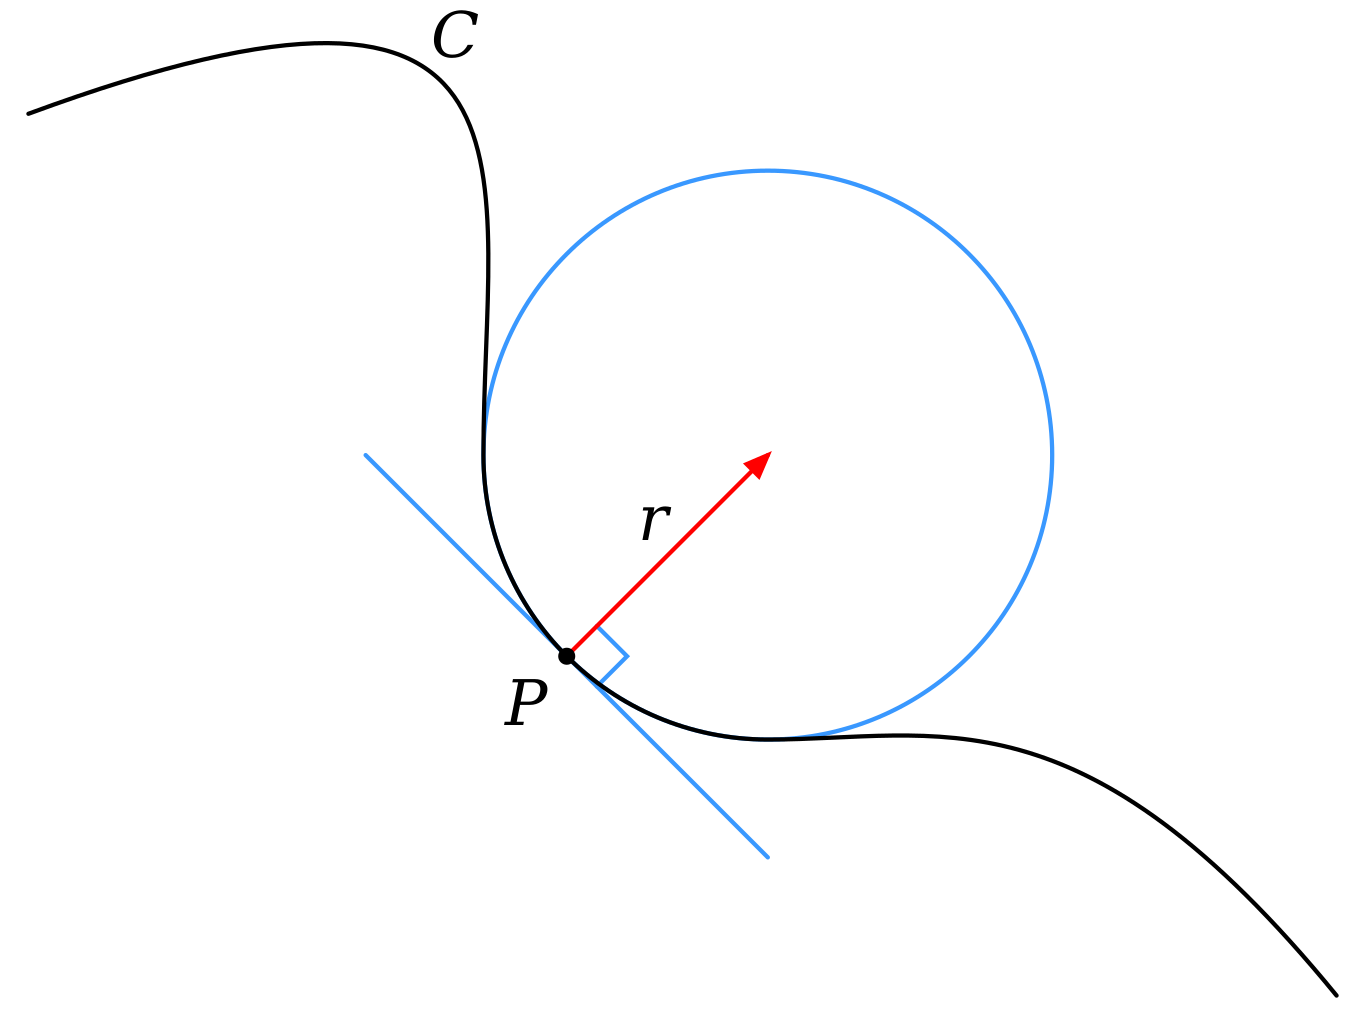
\includegraphics[scale=0.1]{minimal/Kruemmungsradius.png}
  \caption{Krümmungsradius} 
\end{figure}


Zur numerischen Charakterisierung der Krümmung einer Fläche in der Mathematik werden hauptsächlich zwei Grössen benutzt.
Zum einen die Gauss Krümmung was eine intrinsische Krümmung ist und zum andern die Mittlere Krümmung bei welcher es sich um eine extrinsische Krümmung handelt. Bei Minimalflächen ist vor allem die Mittlere Krümmung von Bedeutung, da diese dort null ist.

\index{Gauss Krümmung}

Die Gauss Krümmung einer Fläche im Punkt P ist definiert als das Produkt der zwei Hauptkrümmungen k1 und k2.

\begin{equation} \label{Gauss Krümmung}
  K=k1*k2=1/R1*1/R2
\end{equation}



Die Gauss Krümmung ist eine intrinsische Krümmung. Diese ist  ein Mass für die innere Krümmung einer Fläche. 
Eine gute Vorstellungshilfe ist die Ameisenperspektive. 
Wenn die Ameise auf einer Kugel ist kann sie feststellen, dass nur schon in ihrem kleinen Blickfeld die Winkelsummen eines Dreiecks auf der Oberfläche grösser als 180° ist, demzufolge besitzt die Kugel eine positive Gauss Krümmung. Anders sieht es aus bei einem Zylinder dort misst die Ameise auf der Zylinderoberfläche genau 180° Winkelsumme, das heisst die Gauss Krümmung eines Zylinders ist null.

\index{Mittlere Krümmung}

Die Mittlere Krümmung einer Fläche im Punkt P ist definiert durch den Mittelwert der zwei Hauptkrümmungen k1 und k2.

\begin{equation} \label{Mittlere Krümmung}
  H=1/2*(k1+k2)= (1/2)*(1/R1+1/R2)
\end{equation}

Die Mittlere Krümmung ist eine extrinsische Krümmung. 
Im Gegensatz zur intrinsischen Krümmung kommt es bei einer extrinsischen Krümmung auf die Umgebung an. 
Man kann sich vorstellen, dass man zum Beispiel die Krümmung eines Zylinders (zweidimensionales Objekt) von aussen, also in einem dreidimensionalen Raum betrachtet. 
Ein Zylinder ist aus der Ameisenperspektive flach, schaut man von aussen sieht er jedoch gekrümmt aus.
Dies weil er eine positive mittlere Krümmung aufweist. 
Anders sieht es zum Beispiel bei einer Sattelfläche (Pringels-Chips artigen Fläche) dort ist die Gausskrümmung ungleich null, hingegen kann die Mittlere Krümmung im Spezialfall, dass $R1=-R2$ gleich null sein. In diesem Fall ist diese Sattelfläche ein Beispiel für eine Minimalfläche.

\begin{figure} [H]
  \centering
  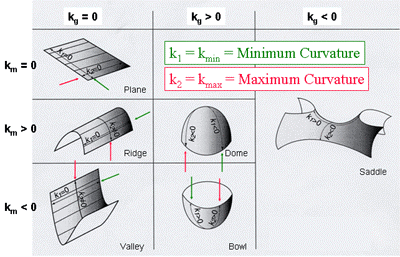
\includegraphics[scale=1]{minimal/Gauss_und_Mittlerekruemmung.png}
  \caption{Vergleich Grauss und Mittlerkrümmung} 
\end{figure}

% \printbibliography[heading=subbibliography]
% \end{refsection}


\section{Defintion der Minimalfläche}
\index{Definition der Minimalfläche}

Um den Begriff der Minimalfläche greifbarer zu gestalten werden hier verschiedene Definitionen, die zueinander gleichwertig sind, erörtert.

\subsection{Variationsproblem}

Def: Eine Fläche $ \textit{M} \subset \mathbf{R}^{3} $ ist genau dann minimal wenn in allen Punkten $p \in M$ die Mittlere Krümmung $=0$ ist.\\
Nach der Definition der Mittleren Krümmung \ref{eq:2} bedeutet dies, dass in jedem Punkt $p$ sich die Krümmungen $k1$ und $k2$ aufheben.
Folglich entspricht eine Minimalfläche der Geodäte im zwei Dimensionen. Zwei Punkte $P1$ und $P2$ können auf der Fläche über eine kürzeste Strecke verbunden werden.  Dies ist sogleich die erste und in diesem Buch wichtigste Definition der Minimalfläche.

\subsection{Lokale Minimalfläche}

Def: Eine Fläche $ \textit{M} \subset \mathbf{R}^{3} $ ist genau dann minimal wenn alle Punkte $ p \in M $ in der Umgebung  im Verhältnis zum Rand am wenigsten Fläche hat.

In anderen Worten ist eine Fläche minimal wenn deren Teilflächen beliebiger grösse ebenfalls minimal sind.  

\subsection{Seifenfilm}

Def: Eine Fläche $ \textit{M} \subset \mathbf{R}^{3} $ ist genau dann minimal wenn jeder Punkt $p \in M$ eine Umgebung mit Rand $D_p$ gleich dem idealem Rand eines Seifenfilms $\partial D_p$ hat.

In diesem Fall ist die Krümmung eines Seifenfilms proportional zum Druckunterschied auf beiden Seiten der Fläche. Die unterschiedlichen Drücke verformen dabei den Film bis auf beiden Seiten der gleiche Druck vorherrscht. Dies kann beispielsweise mit Seife auf einem Drahtgeflecht visualisiert werden. Seifen\textit{blasen} sind nach dieser Definition keine MF, da sie zum Erhalt ihrer Form einen höheren Innendruck haben.

\begin{figure}[H]
  \centering
  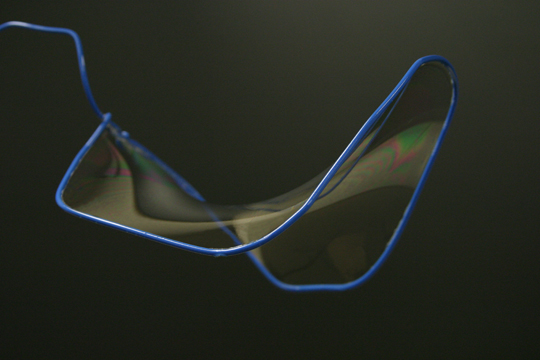
\includegraphics[scale=0.6]{minimal/SoapFilm.jpg}
  \caption{Seifenfilm bildet Minimalfläche} 
\end{figure}

\subsection{Energie}
Def: Eine Fläche $M \subset \mathbf{R}^{3}$ ist genau dann minimal wenn jeder Punkt $p \in M$ eine Umgebung mit minimaler Energie hat.\\
Äquivalent wie die Kettenlinie, welche die Kräfte zwischen den Kettengliedern minimiert, minimiert eine Minimalfläche die "Spannungen" zwischen den Punkten. Stellt man sich die Fläche als dünne Kautschuk-Haut vor, sieht man schnell, dass die einzelnen Kohlenstoff-Ketten die Kräfte innerhalb des Materials ausgleichen und gleichmässig aufteilen. Dies geschieht insbesondere durch die Van der Waals Kräfte zwischen den Kohlenstoff-Ketten.

\begin{figure}[H]
  \centering
  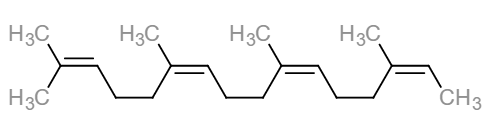
\includegraphics[scale=1]{minimal/cis-Polyisopren.PNG}
  \caption{Kohlenstoffkette von Naturkautschuk} 
\end{figure}


\section{Beispiele}
\index{Beispiele}
\subsection{Katenoid}
Wen man zwei drahtringe parallel zueinander in Seifenwasser taucht entsteht die Form eines Katanoids. 
Das Katanoid ist eines der einfacheren Beispiele einer Minimalfläche. 
In diesem Abschnitt wird die mathematische Berechnung des Katanoids mithilfe der Eulerschen Differenzialgleichung der Variationsrechnung beschrieben.
\begin{figure}[H]
  \centering
  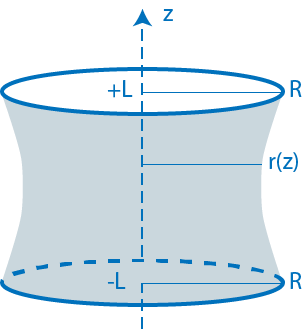
\includegraphics[scale=1]{minimal/soap_film_catanoid.PNG}
  \caption{Skizze: Katanoid} 
\end{figure}
In obiger Skizze ist ein Katanoid abgebildet bei welchem in Bezug auf sie $z$ Achse, der untere Drahtring bei $-L$ und der obere bei $+L$ ist. 
Die beiden Kreise sollen die gleichen Radien haben also gilt $r(-L)=r(+L)=R$. Die flächenpunkte des Katanoids werden mit der Funktion $r(z)$ beschrieben. 
Die Distanz vom Ursprung zu einem Flächenpunkt kann nach Pythagoras mit $s^2=z^2+r^2$ berechnet werden, also gilt auch $ds^2=dz^2+dr^2$.
Formt man diese Gleichung um erhält man die Gleichung \eqref{ds}.

\begin{equation} \label{ds}
  ds=\sqrt{dz^2(1+\frac{dr^2}{dz^2})}= \sqrt{dz^2(1+\dot r^2)}=\sqrt{(1+\dot r^2)}dz
\end{equation}
\subsubsection{Minimalfläche}
Der Seifenfilm versucht automatisch sich im minimalenergetischen Zustand zu befinden. In diesem Zustand ist dann auch die Fläche $S$ des Seifenfilms minimal.
Demzufolge muss das integral \eqref{S1} minimiert werden. 
\begin{equation} \label{S1}  
  S= \int 2 \pi r ds 
\end{equation}
Durch einsetzen von Gleichung \eqref{ds} erhält man die Gleichung \eqref{S2}, welche man als Funktion $F(r,\dot r, z)$ noch verallgemeinert schreiben kann.
\begin{equation} \label{S2}
  S=2 pi \int_{-L}^{+L} r\sqrt{(1+\dot r^2)}dz =2 \pi \int_(-L)^(+L) F(r,\dot r, z) dz 
\end{equation}


Um dieses Integral \eqref{S2} zu minimieren kann man sich der Eulerschen Differenzialgleichung der Variationsrechnung bedienen. 
\subsubsection{Variationsrechnung}
Die Eulerschen Differenzialgleichung der Variationsrechnung wird hier nicht bewiesen nur die anwendungsweise erläutert.
Hat man ein kompliziertes Integral welches man nicht einfach fundamental lösen kann um die Extremwerte zu bestimmen kann man die Eulersche DGL anwenden. Diese besagt, dass anstelle des Ausrechnens eines einer Integralfunktion der Art \eqref{E_DGL1} kann auch die DGL \eqref{E_DGL2} gelöst werden um die Extremwerte solcher Funktionen zu finden.

\begin{equation} \label{E_DGL1}  
  I(y)= \int_a^b F(x,y(x),\dot y(x))dx       
\end{equation}

\begin{equation} \label{E_DGL2}
\left(\frac{\partial F}{\partial y}\right)- \frac{d}{dx} \left(\frac{\partial F}{\partial \dot{y}}\right)=0         
\end{equation}

Für die Gleichung des Katanoids \eqref{S2} erhält man somit die DGL \eqref{K_DGL1}.
\begin{equation} \label{K_DGL1}
\left(\frac{\partial F}{\partial r}\right)- \frac{d}{dz} \left(\frac{\partial F}{\partial \dot{r}}\right)=0    
\end{equation}

Die Gleichung \eqref{K_DGL_H} wird nun schrittweise umgeformt bis eine  Differentialgleichung zweiter Ordnung \eqref{K_DGL_R} entsteht.
\begin{equation} \label{K_DGL_H}
\sqrt{1+{\dot {r}}^2}-\frac{ d }{ dx } \left( r \frac{ 1 }{2  }\left( {1+{\dot {r}}^2}  \right)^{-1/2} 2 \dot {r}\right)=0
\\
\left(1+{\dot {r}}^2  \right)^{-1/2}-(r \frac{ -1 }{2  } \left({1+{\dot {r}}^2}  \right)^{-3/2} 2 \dot{r} \ddot{r}  \dot{r}+ r \left({1+{\dot {r}}^2}  \right)^{-1/2} \ddot{r} +\dot{r} \left({1+{\dot {r}}^2}  \right)^{-1/2} \dot{r}=0
\end{equation}

\begin{equation} \label{K_DGL_R}
1+{\dot {r}}^2=r  \ddot{r}
\end{equation}
\subsubsection{Berechnen}
Die Differenzialgleichung zweiter Ordnung \eqref{K_r} kann mit Hilfe eini-ger mathematischer Umformungen, Aufleiten und hyperbolische Trigonometrie berechnet werden.

\begin{equation} \label{K_r}
r=K cosh(\frac{z-\xi}{K})
\end{equation}

Bei $z=+_L$ ergibt sich \eqref{K_rL}.
\begin{equation} \label{K_rL}
K cosh(\frac{L-\xi}{K})=K cosh(\frac{-L-\xi}{K})
\end{equation}

Da der $cosh$ eine gerade Funktion ist, kommt man entweder auf $L-\xi=-L-\xi$ oder auf $L-\xi=-(L-\xi)$.
Beim ersten Fall wäre $L=-L$ was keinen Sinn ergibt da dann die Fläche gleich Null währe. Beim zweiten Fall muss $\xi=0$ sei also ist die Lösung für das Katanoid die Funktionsgleichung \eqref{K_rz}.

\begin{equation} \label{K_rz}
r(z)=K cosh(\frac{z}{K})
\end{equation}





\subsection{Young–Laplace - Oberflächenspannung}
